%% \documentclass{report}
%% \usepackage{fullpage}
%% \usepackage{tikz}
%% \usepackage[utf8]{inputenc}
%% \usepackage[OT1]{fontenc}

%% \begin{document}

\begin{tikzpicture}

%registres
\draw (8,0) -- (7,-2) -- (9,-2) -- (8,0);
\node at (8,-1.35) {\Large Reg.};

%cache L1
\draw (7,-2) -- (6.5,-3) -- (9.5,-3) -- (9,-2);
\node at (8,-2.5) {\Large Cache L1};

%cache L2
\draw (6.5,-3) -- (6,-4) -- (10,-4) -- (9.5,-3);
\node at (8,-3.5) {\Large Cache L2};

% cache L3
\draw (6,-4) -- (5, -6) -- (11,-6) -- (10,-4);
\node at (8, -5) {\Large Cache L3};

%mémoire
\draw (5,-6) -- (4,-8) -- (12,-8) -- (11,-6);
\node at (8,-7) {\Large Mémoire};

%disque
\draw (4,-8) -- (3,-10) -- (13,-10) -- (12,-8);
\node at (8,-9) {\Large Stockage de masse};


\newcommand{\myarrowup}[4]{% x depart, y depart, longueur
\draw[#4,fill=#4] (#1+0.25,#2) -- (#1+0.25,#2+#3-0.5) -- (#1+0.5,#2+#3-0.5) -- (#1,#2+#3) -- (#1-0.5,#2+#3-0.5) -- (#1-0.25,#2+#3-0.5) -- (#1-0.25,#2) -- (#1+0.25,#2);
}
\newcommand{\myarrowdown}[4]{% x depart, y depart, longueur
\draw[#4,fill=#4] (#1+0.25,#2) -- (#1+0.25,#2-#3+0.5) -- (#1+0.5,#2-#3+0.5) -- (#1,#2-#3) -- (#1-0.5,#2-#3+0.5) -- (#1-0.25,#2-#3+0.5) -- (#1-0.25,#2) -- (#1+0.25,#2);
}

\myarrowdown{0}{0}{10}{white}


\only<4->{
%cout
\myarrowup{1}{-10}{10}{red!50}
\node[rotate=90] at (1,-5) {\Large Prix du bit};
\node at (1,-9.5) {\Huge -};
\node at (1,-0.5) {\Large +};
}

\only<3->{
%taille
\myarrowdown{0}{0}{10}{blue!25}
\node[rotate=90] at (0,-5) {\Large Taille};
\node at (0,-9.5) {\Large +};
\node at (0,-0.5) {\Huge -};
}

\only<2->{
%rapidité
\myarrowup{2}{-10}{10}{teal!50}
\node[rotate=90] at (2,-5) {\Large Rapidité de l'accès aux données};
\node at (2,-9.5) {\Huge -};
\node at (2,-0.5) {\Large +};
}



%% \foreach \i in {0,...,15} {
%%   \foreach \j in {-20,...,0} {
%%     \node[black!25] at (\i,\j) {\i,\j};
%%   }
%% }

\end{tikzpicture}

%\end{document}
